\clearpage\begingroup\SourceLeaf{25b}\HistoricalHead{20}{L}{PHYSIK. BRIEFWECHSEL.}
\begin{center}
[3.]\\[.7em]
\textsc{Gauss} an \textsc{Olbers}. Göttingen, 31. Januar 1829.
\par\medskip\rule{\textwidth}{.35pt}\par
{\small [\textsc{Wilhelm Olbers}, Sein Leben und seine Werke II, 2, 1910, S. 517 ff.]}\par
\rule{\textwidth}{.35pt}
\end{center}
\noindent .\ .\ .\ .\ .\ .\ .\ .\ .\ .\ .\ .\ .\quad Ich bin dabei auf die Theorie der Capillaraction
zurückgekommen, zu deren Behandlung aus einem neuen Gesichtspunkte sich
mir schon vor mehrern Jahren eigenthümliche Ideen dargeboten hatten. Die
Theorie scheint mir dadurch an Einfachheit bedeutend zu gewinnen und die
Mangelhaftigkeit der \textsc{Laplace}schen Theorie gehoben zu werden. Letztere
ist uns den Beweis des Hauptsatzes, dass der Berührungswinkel der Flüssigkeit
an der Wand des Gefässes constant [ist], d. i. bloss von dem Verhältnisse
der Anziehungskraft, die die Theile des Gefässes auf die Flüssigkeit ausüben,
zu der Anziehungskraft der erstern gegen einander abhängt, schuldig
geblieben.

Von der erwähnten Eigenschaft habe ich schon seit Jahr und Tag einen
Gebrauch in der praktischen Astronomie gemacht. Sie wissen, dass ich schon
seit mehrern Jahren den Nullpunkt des Meridiankreises durch Einrichten auf
das Nadir bestimme, wo das Bild des Fadennetzes von einer Quecksilberfläche
reflectirt gesehen wird. Ist hier das Gefäss kleiner als das Objectiv, so geht
offenbar ein Theil des Lichts schon deshalb verloren, allein ein noch grösserer
Theil dadurch, dass vermöge der Capillaraction das Quecksilber selbst in einer
bedeutenden Entfernung vom Rande merklich von der Plangestalt abweicht
(Figur 1 [auf S. 21]). Ich vermeide diess, indem ich mich eines Gefässes bediene,
dessen innere Fläche oben conisch, nach oben zu sich verengend, ich
habe ausdrehen lassen, ungefähr unter einem Winkel von \(45^{0}\).

In diesem Gefäss ist die Oberfläche des Quecksilbers ohne die geringste
merkliche Convexität. Man könnte von dieser Idee auch in manchen anderen
Fällen vortheilhaften Gebrauch machen. Man kann übrigens jenen Zweck
\clearpage\SourceLeaf{26}\HistoricalHead{21}{R}{GAUSS AN OLBERS.}
\noindent auch ziemlich erreichen, wenn man das Quecksilber in eine sehr flache goldene
Schale schüttet, oder in eine andere anquickungsfähige.
\begin{center}
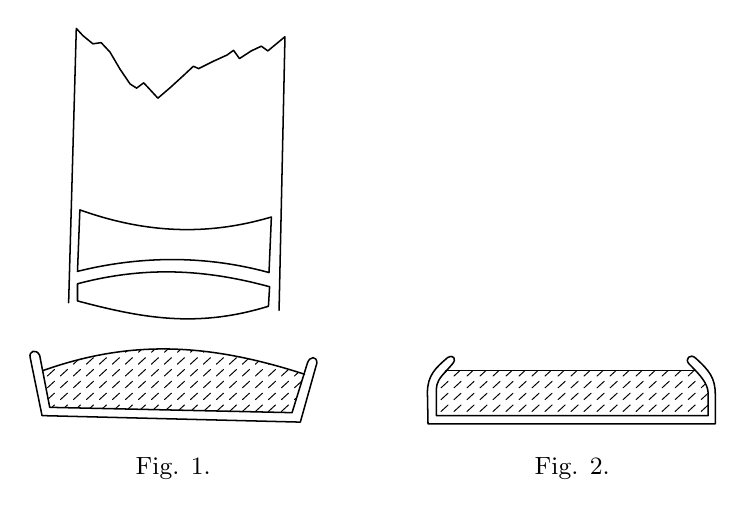
\begin{tikzpicture}[x=.0075cm,y=-.0075cm,line width=.55pt,line cap=round,line join=round]
\draw (123,490)--(136,26)--(147,38)--(164,52)--(178,50)--(193,66)--(210,95)--(227,120)--(238,127)--(250,118)--(263,132)--(274,144)--(295,126)--(318,105)--(334,90)--(343,94)--(369,81)--(391,71)--(402,63)--(412,77)--(432,64)--(449,56)--(460,64)--(489,40)--(479,503);
\draw (142,333)..controls (243,369) and (348,380)..(466,345)--(462,439)..controls (349,408) and (238,412)..(138,437)--cycle;
\draw (138,458)..controls (251,428) and (353,433)..(463,463)--(461,496)..controls (338,534) and (244,515)..(138,487)--cycle;
\begin{scope}
\clip (79,605)..controls (220,555) and (350,555)..(522,611)--(501,676)--(91,667)--cycle;
\foreach \y in {574,594,614,634,654,674}{\foreach \x in {65,87,...,535}{\draw[line width=.35pt] (\x,\y)--++(12,-11);}}
\end{scope}
\draw (79,605)..controls (220,555) and (350,555)..(522,611);
\draw (78,681)--(58,583)..controls (55,572) and (68,567)..(74,579)--(91,667)--(501,676)--(527,592)..controls (531,580) and (543,580)..(543,592)--(515,692)--cycle;
\begin{scope}
\clip (745,681)--(745,638)..controls (745,622) and (753,614)..(761,605)--(1182,605)..controls (1197,615) and (1204,629)..(1205,643)--(1205,681)--cycle;
\foreach \y in {614,634,654,674,694}{\foreach \x in {731,753,...,1220}{\draw[line width=.35pt] (\x,\y)--++(12,-11);}}
\end{scope}
\draw (761,605)--(1182,605);
\draw (731,695)--(730,642)..controls (730,613) and (744,600)..(764,583)..controls (774,577) and (780,585)..(772,594)--(755,613)..controls (745,625) and (745,632)..(745,643)--(745,681)--(1205,681)--(1205,643)..controls (1204,626) and (1192,613)..(1173,594)..controls (1164,585) and (1175,575)..(1184,584)..controls (1207,605) and (1217,617)..(1217,646)--(1217,695)--cycle;
\node[font=\small,anchor=north] at (300,735) {Fig. 1.};
\node[font=\small,anchor=north] at (975,735) {Fig. 2.};
\end{tikzpicture}
\end{center}
\noindent\hspace*{\parindent}Bei Gelegenheit jener Untersuchungen, die nicht wohl einen Auszug hier
zulassen, bin ich neulich auf ein neues mechanisches Grundprincip gekommen,
welches ich Ihnen doch anzeigen will. Bekanntlich verwandelt zwar schon
das Princip der virtuellen Geschwindigkeiten die ganze Statik in eine mathematische
Aufgabe, und durch d’\textsc{Alemberts} Princip für die Mechanik ist diese
wieder auf die Statik zurückgeführt. Es liegt daher in der Natur der Sache,
dass es kein neues Grundprincip geben kann, das nicht der Materie nach in
jenen beiden enthalten und aus ihnen abzuleiten wäre. Inzwischen scheint
mir doch durch diesen Umstand nicht jedes neue Grundprincip werthlos zu
werden. Das Princip der virtuellen Geschwindigkeiten ist allerdings unschätzbar,
allein mir deucht, es hat das Eigenthümliche, dass es sich den Beifall
erst bei näherer Bekanntschaft erwirbt, und dass es jedem, wenn er es zum
\textls[120]{erstemahl kennen lernt}, den Eindruck von Verwunderung macht, dass die
Natur sich ein Gesetz aufgelegt hat, an dem man sein Creditiv gewiss
nicht gleich erkennt. Zweitens ist es zwar allerdings dem natürlichen historischen
Gange der Ausbildung der Wissenschaft selbst und der Ausbildung
des Individuums (Anfängers) ganz angemessen, dass die Statik der Mechanik
vorangehe, und diese auf jene begründet werde; aber aus einem \textls[120]{höhern}
Standpunkte betrachtet sollte es, meine ich, doch gerade umgekehrt sein,
indem die Statik nichts ist als ein ganz specieller Fall der Mechanik.

Ich finde nun, dass alles sich in ein höchst einfaches Gesetz zusammen-\clearpage\SourceLeaf{27}\HistoricalHead{22}{L}{PHYSIK. BRIEFWECHSEL.}
\noindent fassen lässt, oder wenn Sie lieber wollen in zwei, indem ich Ein triviales
vorausschicke:
\par\noindent\hspace*{\parindent}1) Die Bewegung eines \textls[120]{freien} materiellen Punktes in jedem unendlich
kleinen Zeittheilchen ist aus den einzelnen Bewegungen, die er theils in Folge
der Trägheit nach seiner im Anfang des Zeittheilchens Statt findenden Geschwindigkeit
und Richtung, theils in Folge der einzelnen auf ihn einwirkenden
Kräfte haben wird, zusammengesetzt.
\par\noindent\hspace*{\parindent}2) Wenn die Bewegung eines Systems von materiellen Punkten nicht
frei, sondern durch gegenseitige Relationen oder durch äussere Hindernisse
beschränkt ist, so liegen die Plätze, wo sie nach einem unendlich kleinen
Zeittheilchen wirklich sich befinden, denen, wo sie [sich] in Folge einer freien
Bewegung befinden müssten, \textls[120]{so nahe wie möglich}. Dies so nahe wie
möglich ist gerade eben so zu verstehen, wie bei der Darstellung von Erfahrungen,
die zufällige Fehler involviren. Nemlich: Es sein \(m,m',m''\) u.s.w.
die materiellen Punkte; \(p,p',p''\) u.s.w. die Plätze des Raums, wo sie zu Anfang
eines unendlichkleinen Zeitraums sich befinden; \(q,q',q''\) u.s.w. die Plätze,
wo sie sich am Ende des Zeitraums befinden würden, falls sie sich alle frei
bewegen könnten; \(r,r',r''\) u.s.w. die Plätze, wo sie sich am Ende des Zeitraums
wirklich befinden; \(R,R',R''\) u.s.w. \textls[120]{indefinite} Plätze, wo sie sich
unbeschadet der beschränkenden Bedingungen gleichzeitig befinden können
(so dass \(p,p',p''\) u.s.w. wie auch \(r,r',r''\) u.s.w. sich unter dem allgemeinen
\(R,R',R''\) u.s.w. befinden, nicht aber \(q,q',q''\) u.s.w.); dann ist das Aggregat
\[
 m(qr)^2+m'(q'r')^2+m''(q''r'')^2+\text{u.s.w.}
\]
\noindent ein Minimum, d. i. das kleinste aus allen
\[
 m(qR)^2+m'(q'R')^2+m''(q''R'')^2+\text{u.s.w.}
\]

Dieser vollkommene Parallelismus zwischen den Auswegen, welche einerseits
die Natur und andererseits der rechnende Geometer — jedes bei seinem
eigenthümlichen Geschäft — in Collisionsfällen einschlagen, hat mir viel Vergnügen
gemacht. Es bedarf keiner Bemerkung, dass im Fall des Gleichgewichts
\[
 m(qp)^2+m'(q'p')^2+m''(q''p'')^2+\text{u.s.w.}
\]
\noindent selbst das Minimum ist.
\par\noindent\makebox[\textwidth][s]{.\hfill .\hfill .\hfill .\hfill .\hfill .\hfill .\hfill .\hfill .\hfill .\hfill .\hfill .\hfill .\hfill .\hfill .\hfill .\hfill .\hfill .\hfill .\hfill .\hfill .\hfill .\hfill .\hfill .\hfill .\hfill .\hfill .}
\begin{center}\rule{.25\textwidth}{.35pt}\end{center}
\clearpage\endgroup
